\chapter{Manual de instalación y uso}
\label{appendix:manual}

Manual de instalación y uso de la solución del trabajo (\ref{chap:poc}). Estos pasos han sido probados en un sistema \verb|Ubuntu 19.04| de 64 bits.

\section{Prerequisitos}

\subsection{SEAL}

Como hemos comentado, Microsoft SEAL no necesita ninguna dependencia. Para instalarlo (generar las librerías y los archivos de cabeceras) seguimos los siguientes pasos:

\begin{minted}{console}
$ git clone https://github.com/Microsoft/SEAL
$ cd SEAL/native/src
$ cmake .
$ make
\end{minted}

Generará la librería compilada en la ruta \verb|SEAL/native/lib|, y tendremos sus archivos \verb|.h| en el directorio \verb|SEAL/native/src|.

Para más detalles, ver la guía de instalación oficial en \url{https://github.com/Microsoft/SEAL}.

\subsection{TFHE}

La librería TFHE sí que tiene algunos prerequisitos, que satisfaremos ejecutando:

\begin{minted}{console}
$ sudo apt-get install build-essential cmake cmake-curses-gui
\end{minted}

Una vez instalados, descargamos el código y lo configuramos para compilarlo:

\begin{minted}{console}
$ #clone the tfhe repository
$ git clone --recurse-submodules --branch=master https://github.com/tfhe/tfhe.git
$ cd tfhe
$ #configure the build options
$ mkdir build
$ cd build
$ ccmake ../src
\end{minted}

Abrirá un menú con varias opciones dependiendo de las características que queramos utilizar. En la figura \ref{fig:ccmake_tfhe} se muestran las que hemos utilizado en nuestra instalación.

\begin{figure}[h]
    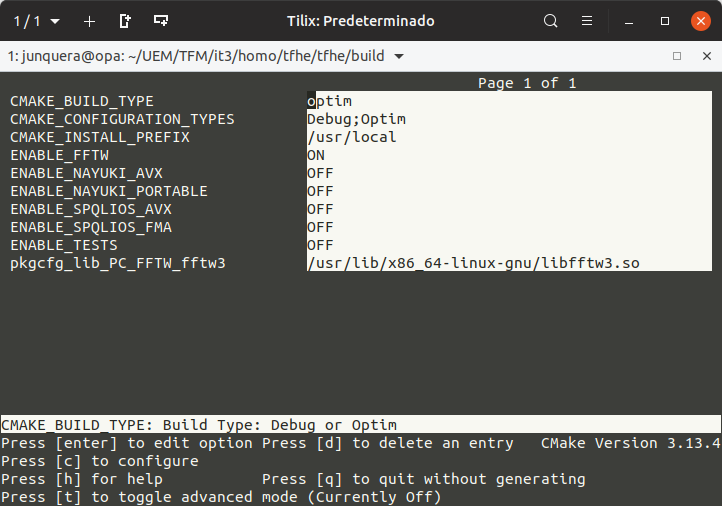
\includegraphics[width=\linewidth]{ccmake_tfhe}
    \caption{Parámetros de configuración de tfhe}
    \label{fig:ccmake_tfhe}
\end{figure}

Tras guardar esta configuración, símplemente ejecutamos:

\begin{minted}{console}
$ #build the library
$ make
\end{minted}

Como resultado obtendremos la librería compilada dentro de \verb|tfhe/build/libtfhe|. En función de los parámetros que hayamos elegido tendrá un nombre u otro. Con nuestros parámetros se llamará \verb|libtfhe-fftw.so|

Para más detalles, ver la guía de instalación oficial en \url{https://tfhe.github.io/tfhe/installation.html}.

\section{Instalación}

\subsection{tfhe-math}

Para instalar \verb|tfhe-math| necesitaremos haber compilado \verb|tfhe|. Primero descargamos el código y entramos en la carpeta para configurarlo:

\begin{minted}{console}
$ git clone git@gitlab.com:junquera/tfhe-math.git
$ cd tfhe-math
\end{minted}

Editamos el archivo \verb|src/Makefile| y especificamos en la variable \verb|TFHE_PREFIX| la ruta en la que están la librería de \verb|tfhe| y sus archivos \verb|.h|. Tras guardar, entramos en la carpeta \verb|src| y ejecutamos el comando \verb|make|. Creará una carpeta llamada \verb|prefix| en la raíz del proyecto con todos los archivos necesarios para que utilicemos la librería en otros proyectos.

\subsection{tfhe-cs}

Descargaremos el código con las funcionalidades de cliente y servidor desde su repositorio en GitLab:

\begin{minted}{console}
$ git clone --recurse-submodules git@gitlab.com:junquera/tfhe-cs.git
$ cd tfhe-cs
\end{minted}

De esta forma, además se descargará la librería \verb|tfhe-math| para que la usemos (si no la hemos instalado aún).

En el archivo \verb|Makefile| tenemos que especificar la ruta a las carpetas de prefix (las carpetas que contengan las librerías y los archivos de cabeceras \verb|.h|) de \verb|tfhe| y de \verb|tfhe-math|.

Ejecutando el comando \verb|make| generaremos el programa cliente, el programa servidor y el ejecutable con los test.

\subsection{seal-cs}

Haremos exactamente lo mismo que con \verb|tfhe-cs|, pero eligiendo su repositorio correspondiente:

\begin{minted}{console}
$ git clone git@gitlab.com:junquera/seal-cs.git
$ cd tfhe-cs
\end{minted}

Esta vez, en lugar de especificar la ruta a \verb|tfhe|, indicamos en el archivo \verb|Makefile| la ruta a \verb|SEAL| y ejecutamos el comando \verb|make|.

\section{Uso}

A continuación veremos los distintos usos que podemos darle a nuestra implementación, ya sea para ejecutar el código del trabajo o realizar nuestra propia implementación. Las cabeceras de referencia de cada programa se pueden ver en el anexo \ref{appendix:cs-headers}.

\subsection{tfhe-math}

Para utilizar las funciones de \verb|tfhe-math| únicamente tenemos que enlazar nuestro código 
con la librería, e incluir sus archivos de cabecera en él. Por ejemplo, para utilizar las funciones aritméticas escribiríamos:

\begin{minted}{c++}
#include "tfhe-math/arithmetic.h"
\end{minted}

Después trabajaríamos con sus métodos, que funcionan tal y como hemos indicado en la sección \ref{tag:tfhe-math-ops}, teniendo en cuenta únicamente que:

\begin{itemize}
    \item Los métodos precedidos con \verb|u_| son más rápidos, pero no tienen en cuenta el sigo.
    \item Si se trabaja con números reales, para multiplicar y dividir usaremos las funciones \verb|multiply_float| y \verb|divide_float| respectivamente (en lugar de \verb|multiply| y \verb|divide|)
\end{itemize}

\subsection{tfhe-cs}

Si quisiésemos usar la funcionalidad del cliente o del servidor (no del programa, si no de la clase) bastaría con utilizar los códigos \verb|client.cpp| o \verb|server.cpp| (respectivamente) incluyendo sus archivos de cabeceras.

\subsection{seal-cs}

Al igual que con \verb|tfhe-cs| podemos utilizar nuestros códigos de cliente y servidor para hacer una implementación propia con sus funcionalidades, o ejecutar los programas generados (\verb|client|, \verb|server| y \verb|test|).